\documentclass{article}
\usepackage[utf8]{inputenc}
\usepackage[T1]{fontenc}
\usepackage{csquotes}
\usepackage[english]{babel}
\usepackage{graphicx} % Required for inserting images
\usepackage{amsmath,mathtools}
\usepackage{bm}
\usepackage[svgnames]{xcolor}
\usepackage{longtable}
\usepackage[section]{placeins}
\usepackage{dirtytalk}

\usepackage{biblatex}
\addbibresource{refs.bib}

\usepackage[pdfencoding=auto, psdextra]{hyperref}
\hypersetup{
    colorlinks,
    linkcolor={blue!50!black},
    citecolor={blue!50!black},
    urlcolor={blue!80!black}
}

\title{Orbital mechanics theory notes}
\author{cxcorp}
\date{August 2023}

\begin{document}

\maketitle

\tableofcontents

\pagebreak

\section{Keplerian orbital elements}

The parameters required to uniquely identify a specific orbit. Assuming a two-body system.

\begin{figure}[htp]
    \centering
    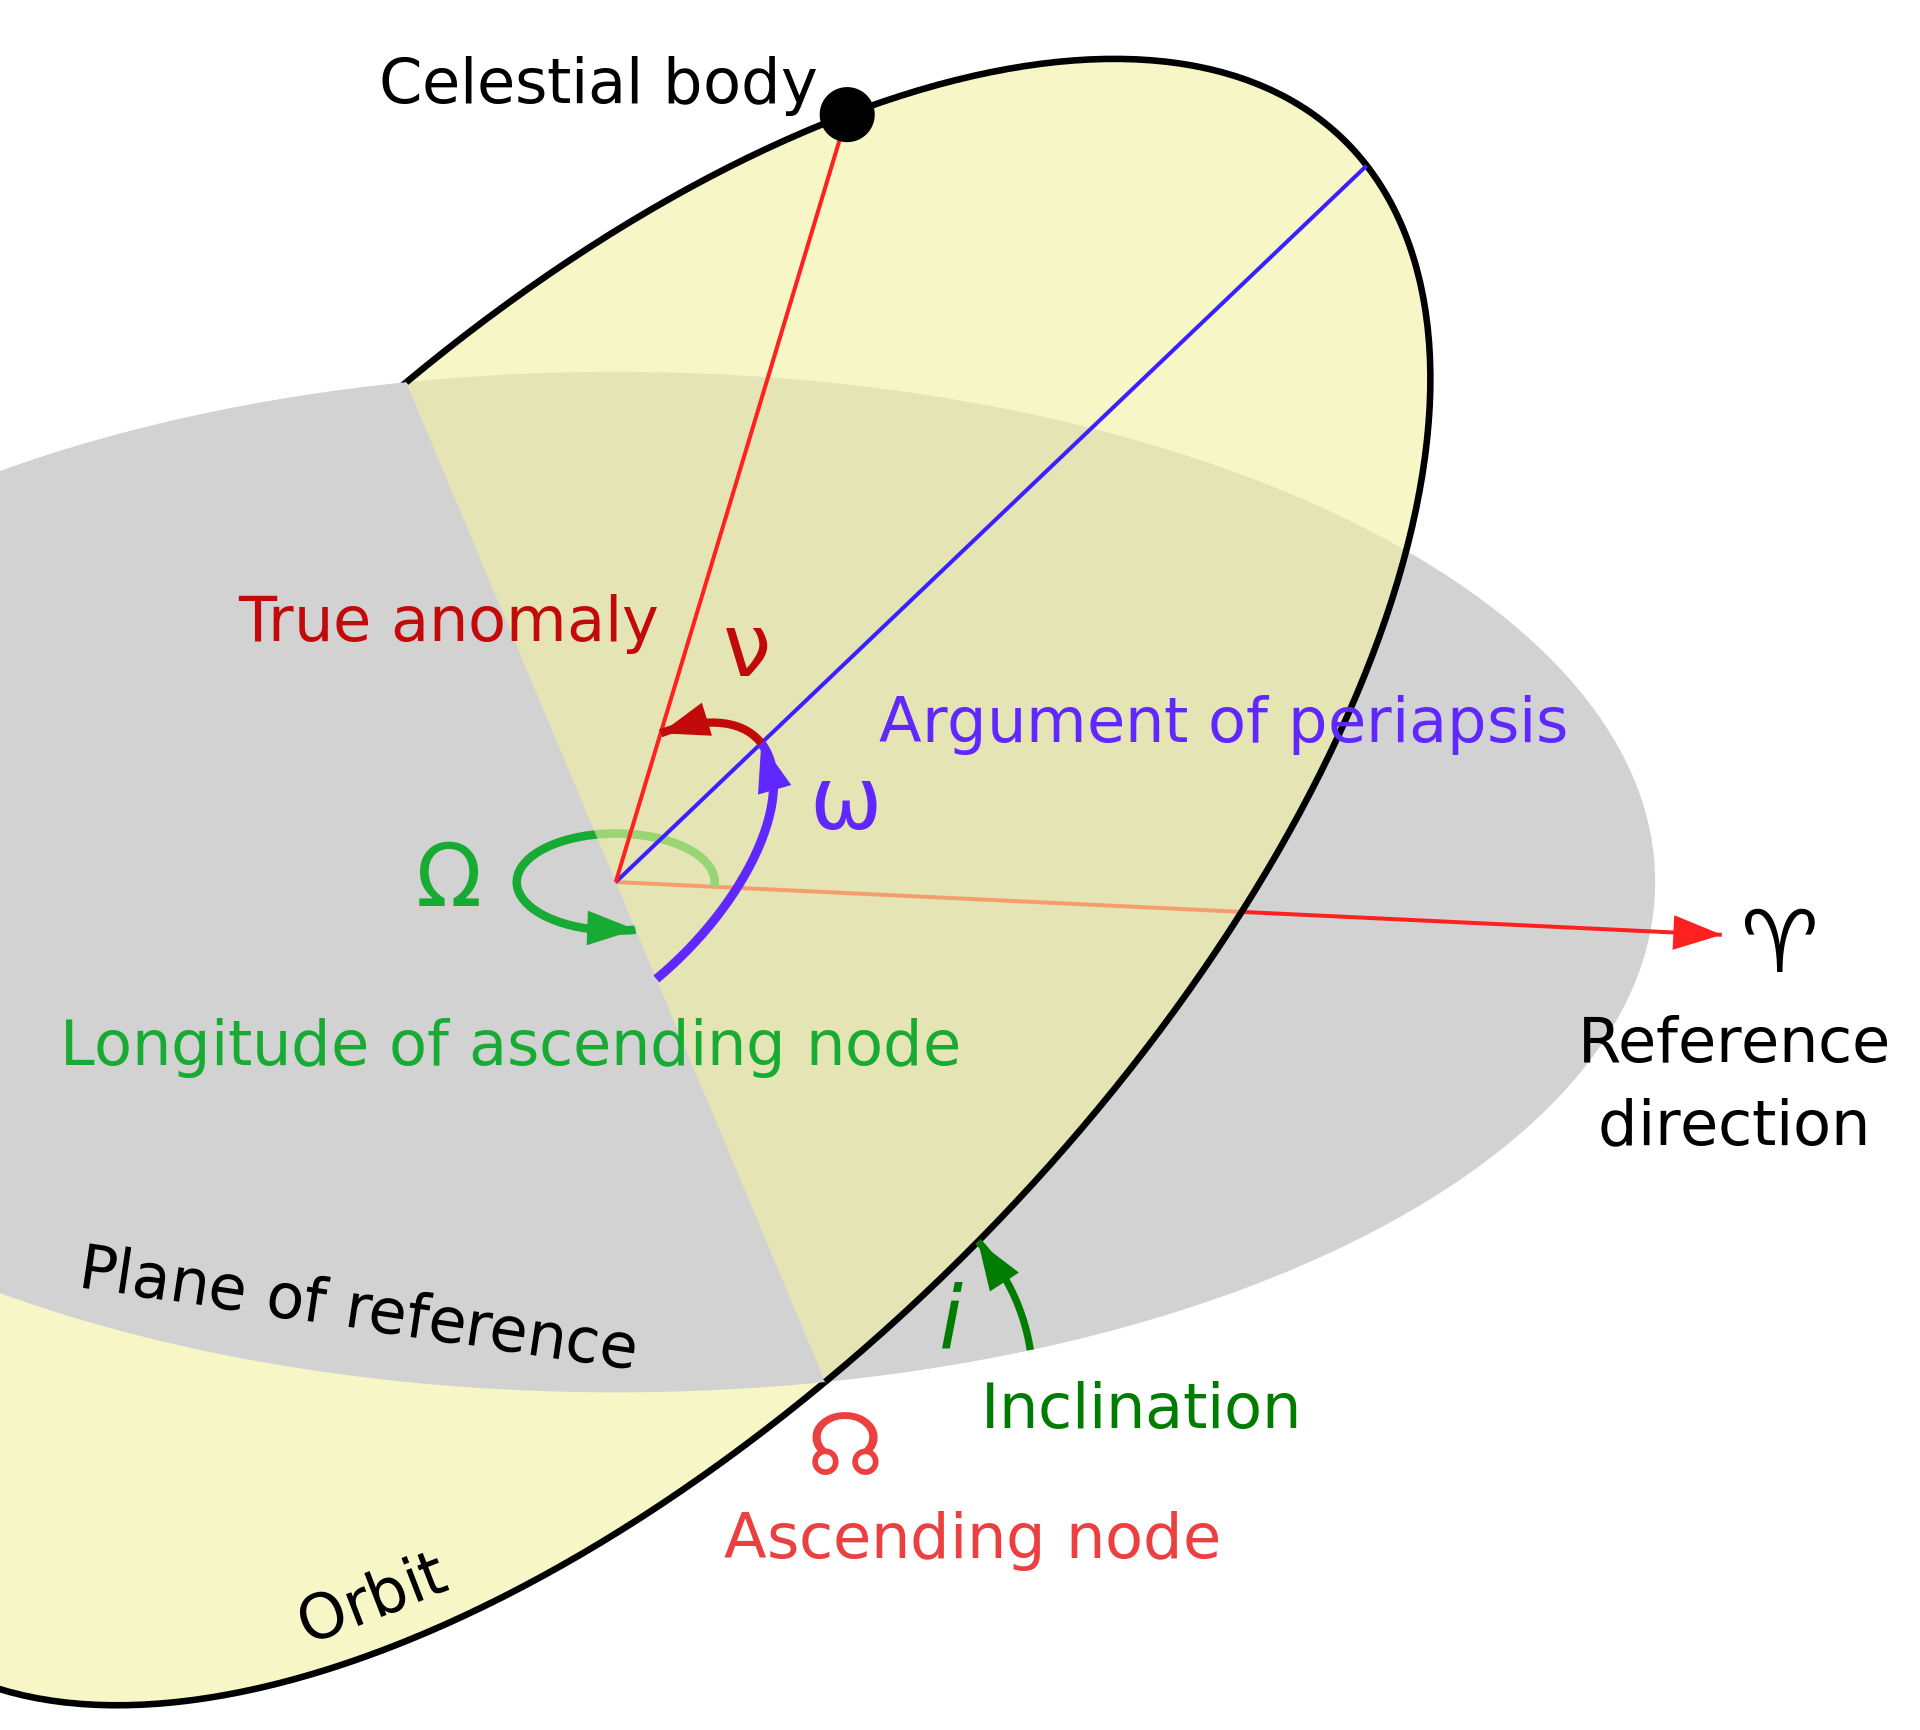
\includegraphics[width=0.7\textwidth]{img/Orbit1.svg.png}
    \caption{Diagram illustrating and explaining various terms in relation to Orbits of Celestial bodies. \\ {\small By \href{https://en.wikipedia.org/wiki/User:Lasunncty}{Lasunncty} at the \href{https://en.wikipedia.org/wiki/}{English Wikipedia}. Licensed under \href{http://creativecommons.org/licenses/by-sa/3.0/}{CC BY-SA 3.0}.}}
\end{figure}




\section{Shape and size of the ellipse}

\subsection{$a$ -- Length of semi-major axis}
\label{sec:semimajor}

The \textbf{major axis} is the longest diameter of an ellipse. The semi-major axis is half of the diameter.

\bigskip

\begin{minipage}{0.45\textwidth}
    \centering
    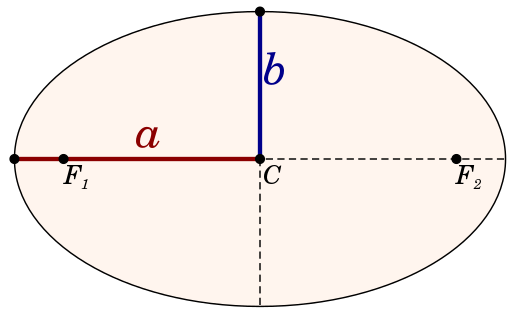
\includegraphics[width=5cm]{img/semimajor.png}
\end{minipage}\hfill
\begin{minipage}{0.45\textwidth}
    \centering
    \begin{align*}
        \Aboxed{\textcolor{DarkRed}{\bm{a}} &= \text{length of semi-major axis}} \\
        b &= \text{length of semi-minor} \\
        c &= \text{center point} \\
        F_1, F_2 &= \text{focus points}
    \end{align*}
\end{minipage}

\subsection{$e$ -- Eccentricity}
\label{sec:eccentricity}

Amount by which orbit deviates from a perfect circle. More $e \Rightarrow \text{more squished}$.

\begin{figure}[htp]
    \centering
    \begin{minipage}{0.5\textwidth}
        \begin{center}
        \begin{tabular}{ |c|c| } 
        \hline
        Eccentricity & Shape \\
        \hline
        \hline
        $e = 0$ & Circular orbit \\ 
        $0 < e < 1$ & Elliptic orbit \\ 
        \hline
        $e = 1$ & Parabolic trajectory \\ 
        $e > 1$ & Hyperbolic trajectory \\ 
        \hline
        \end{tabular}
        \end{center}
    \end{minipage}\hfill
    \begin{minipage}{0.5\textwidth}
        \centering
        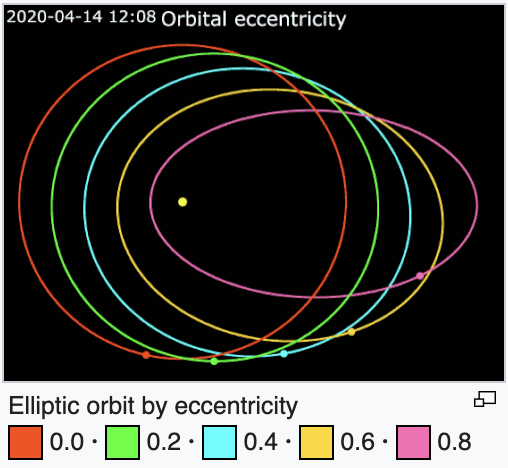
\includegraphics[width=5cm]{img/eccentricity.png}
        \caption{Elliptic orbit by eccentricity. \\ {\small By \href{https://commons.wikimedia.org/wiki/User:Phoenix7777}{Phoenix7777} at the \href{https://en.wikipedia.org/wiki/}{English Wikipedia}. Licensed under \href{https://creativecommons.org/licenses/by-sa/4.0/}{CC BY-SA 4.0}.}}
    \end{minipage}
\end{figure}

\subsubsection{Relation to apoapsis and periapsis}
\begin{minipage}{0.54\textwidth}
    \begingroup
    \addtolength{\jot}{1em}
    \begin{align}
        \Aboxed{& e = \frac{r_a - r_p}{r_a + r_p}} = 1 - \frac{2}{\frac{r_a}{r_p} + 1} \\
        \Leftrightarrow \quad \Aboxed{& r_p = \frac{(1-e)r_a}{1+e}} \\
        \Leftrightarrow \quad \Aboxed{& r_a = -\frac{(1+e)r_p}{e-1}}
    \end{align}
    \endgroup
\end{minipage}\hfill
\begin{minipage}{0.36\textwidth}
    \begin{align*}
        e &= \text{eccentricity} \\
        a &= \hyperref[sec:semimajor]{\text{semi-major axis length}} \\
        r_a &= \text{apoapsis} \\
        r_p &= \text{periapsis}
    \end{align*}
\end{minipage}



\section{Orientation of the orbital plane}

\subsection{$i$ -- Inclination}

\say{vertical tilt of the ellipse with respect to the reference plane, measured at the ascending node (where the orbit passes upward through the reference plane, the green angle i in the diagram \cite{wiki:orbitalelements}}

\subsection{$\Omega$ -- Longitude of the ascending node}
Horizontal tilt. Angle from reference direction to the ascending node.


\section{Other orbital parameters}

\subsection{$T$ -- Orbital period}

How long it takes to complete one orbit.

For all orbits with a specific \hyperref[sec:semimajor]{length of semi-major axis}, the orbital period is the same. The shape of the ellipsis (\hyperref[sec:eccentricity]{eccentricity}) does not matter.

\begin{minipage}{0.5\textwidth}
    \begin{align}
        \Aboxed{& T =  \sqrt{\frac{ \pi^2 \left(r_p+r_a\right)^3 }{ 2\mu }}} = 2 \pi \sqrt{\frac{a^3}{\mu}}
    \end{align}
\end{minipage}\hfill
\begin{minipage}{0.35\textwidth}
    \begin{align*}
        a &= \hyperref[sec:semimajor]{\text{semi-major axis length}} \\
        \mu &= \text{\textit{see below}}
    \end{align*}
\end{minipage}

\bigskip

\cite{kspwiki:orbitmath}.

\subsection{$r\left(\phi\right)$ -- Radius of orbit at specific angle}

This is the distance between the craft and the body \cite{kspwiki:orbitmath} at a specific angle.

\begin{minipage}{0.6\textwidth}
    \begin{align}
        \Aboxed{r\left(\phi\right) = 2 \frac{r_p r_a}{r_p + r_a + (r_a - r_p)\cos{\phi}}}
    \end{align}
\end{minipage}\hfill
\begin{minipage}{0.35\textwidth}
    \begin{align*}
        r_a &= \text{apoapsis} \\
        r_p &= \text{periapsis} \\
        \phi &= \text{orbital angle}
    \end{align*}
\end{minipage}

\subsection{$\mu$ -- Standard gravitational parameter}

Specific to a celestial body. It is the gravitational constant $G$ multiplied by the mass of the body $M$:
\[
\mu = GM
\]

\subsubsection{Standard gravitational parameters of KSP celestial objects}

\begin{center}
    {\renewcommand{\arraystretch}{1.5}
    \begin{longtable}{ |c|c| } 
        \hline
        Celestial object & $\mu \quad (\frac{m^3}{s^2})$ \\
        \hline
        Mun & $6.5138398 \cdot 10^{10}$ \\
        $e > 1$ & Hyperbolic trajectory \\ 
        \hline
    \end{longtable}
    }
\end{center}

\section{todo}

\begin{itemize}
    \item Geosynchronous orbits \cite{kspwiki:geosyncmath}
\end{itemize}



\printbibliography[heading=bibnumbered]

\end{document}
